
%(BEGIN_QUESTION)
% Copyright 2006, Tony R. Kuphaldt, released under the Creative Commons Attribution License (v 1.0)
% This means you may do almost anything with this work of mine, so long as you give me proper credit

Prøveventilen i en gasskromatograf har en svært viktig funksjon: den må injisere et presist prøvevolum i et presist tidsrom. Figuren under viser komponentene i en grunnleggende gasskromatograf. Væskekromatografer skiller seg bare litt fra dette:

$$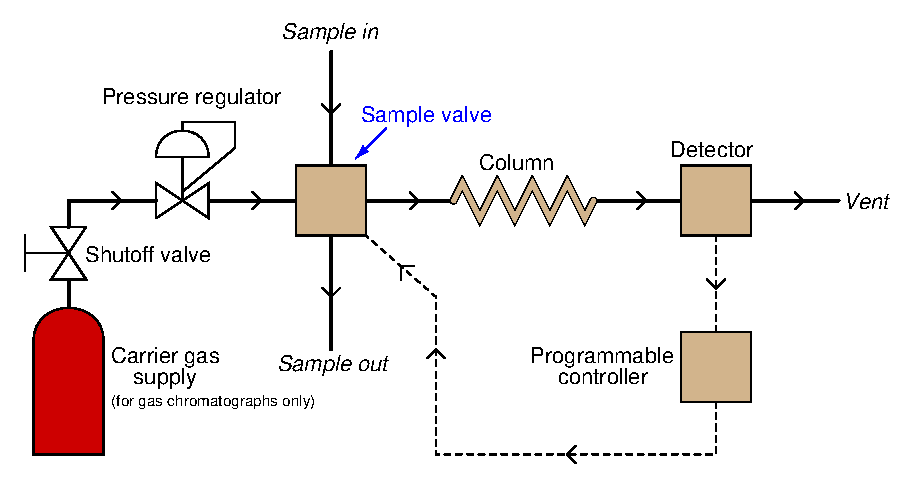
\includegraphics[width=15.5cm]{i00675x01.eps}$$

Siden funksjonen er så viktig, er prøveventilen konstruert annerledes enn vanlige ventiler. De fleste prøveventiler i kromatografer er roterende, med spor i en metallrotor som leder fluidstrømmer langs ulike baner. Et vanlig design bruker seks porter og tre spor, slik:

$$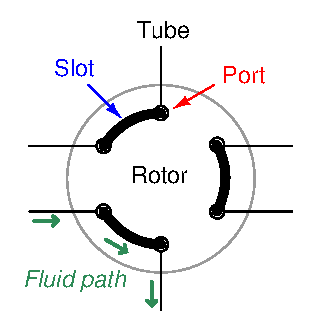
\includegraphics[width=15.5cm]{i00675x03.eps}$$

Illustrasjonen under viser en typisk prøveventil med roterende ventilinnmat i to ulike posisjoner. {\it Loading}-posisjonen klargjør prøvesløyfen for injeksjon mens kolonnen skylles med bæregass. {\it Sampling}-posisjonen injiserer et nøyaktig prøvevolum i kolonnen, etterfulgt av bæregass.

$$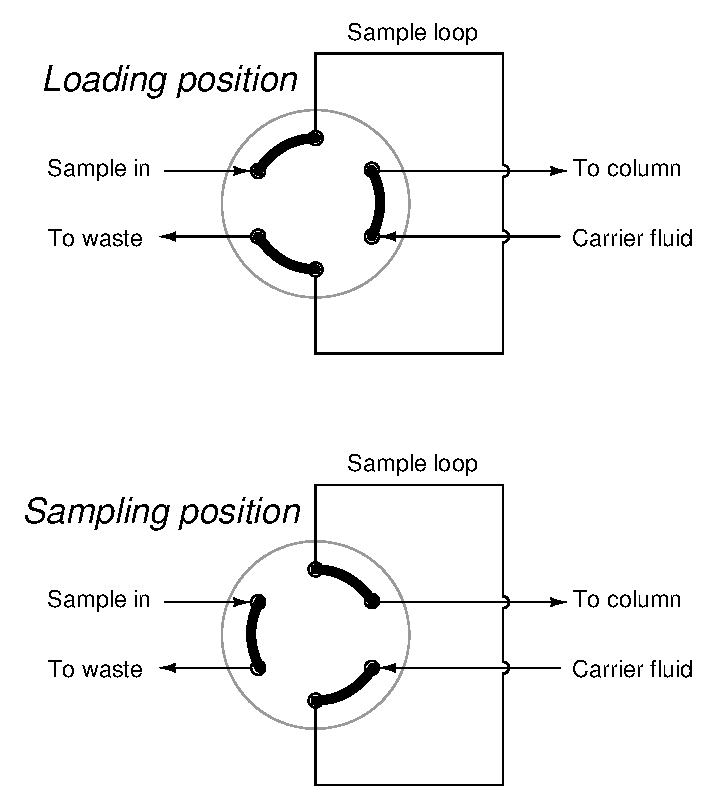
\includegraphics[width=15.5cm]{i00675x02.eps}$$

Forklar hvordan denne ventil- og rørkonfigurasjonen gir et konsistent, målt prøvevolum ved hver injeksjonssyklus. Identifiser også hva som må endres for å doble injisert volum i kolonnen per syklus.

\underbar{file i00675no}
%(END_QUESTION)





%(BEGIN_ANSWER)

Injisert prøvevolum i en kromatograf bestemmes av det interne volumet i prøvesløyferøret {\it pluss} volumet av ett ventilspor. For å doble injisert volum nøyaktig må man derfor øke lengden på prøvesløyferøret med litt mer enn en faktor to.

\vskip 10pt

Prosesskromatografer bruker svært små prøvevolum. Typisk prøvevolum ligger i størrelsesorden titalls {\it mikro}liter.

\vskip 10pt

Hvor lenge prøveventilen står i sampling-posisjon har ingen betydning for injisert volum {\it så lenge tiden overstiger minimumstiden som kreves for å skylle prøvesløyfen og ventilsporet helt tomme}. Enhver tid utover dette er irrelevant. Hvis ventilen står kortere enn denne minimumstiden, blir prøvesløyfen ikke helt tømt, og injisert volum blir lavere enn ønsket.

%(END_ANSWER)





%(BEGIN_NOTES)


%INDEX% Måling, analytisk: kromatografi

%(END_NOTES)
